\section{Prozesssteuerung}
\label{sec:prozesssteuerung}

Nachdem in Kapitel \ref{sec:prozessplanung} eine Benutzeroberfläche zur Prozessplanung entwickelt wurde, muss nun der dahinterliegende Programmcode für die Weitergabe des geplanten Prozesses an die Maschinen und damit der Prozesssteuerung entworfen und implementiert werden. Es gilt nun zunächst, eine geeignete Kommunikationsstruktur auszuarbeiten, welche das Prozessplanungs-Interface an die Fertigungsanlagen anbindet und anschließend müssen die relevanten Teile dieser Infrastruktur implementiert werden.

\subsection*{Architektur und Konzeption}
\label{subsec:prozesssteuerung_architektur}

Die in Kapitel \ref{sec:prozessplanung} genannten Kriterien gelten grundsätzlich auch hier, jedoch muss beachtet werden, dass Nutzer in der Regel nicht direkt mit der in diesem Kapitel behandelten Software interagieren. Einige der nutzerorientierten Kriterien entfallen daher. Da eine Übertragung von Daten hier eine zentrale Rolle spielt, ist die Datensicherheit von erheblicher Bedeutung. Konkret soll neben der Einhaltung europäischer Regelungen wie der Regulation 2018/1725 [\cite{euDataProtectionRegulation}] auch der industrielle Cyber-Sicherheitsstandard IEC 62443 [\cite{IEC62443}] befolgt werden. Selbstverständlich sollen auch Regulationen wie die europäische Regulation zur Verarbeitung personenbezogener Daten [\cite{euDataProtectionRegulation}] eng befolgt werden.

Um nun eine Infrastruktur zur Kommunikation und Steuerung von Fertigungsanlagen an verschiedenen Standorten über einen Web-Browser aufzubauen, sind einige Überlegungen zu beachten:
%
\begin{itemize}
    \item Da die Kommunikation von einem Web-Browser – spezifischer von der in Kapitel \ref{sec:prozessplanung} implementierten Applikation – ausgeht, muss JavaScript oder ein HTML Form genutzt werden.
    \begin{itemize}
        \item Um die zuvor genannten Kriterien zu erfüllen – konkret die Kriterien der Serviceorientierung und der Modularität – sollte eine REST API genutzt werden, welche über ECMAScript 2020 angesprochen wird.
    \end{itemize}
    \item Da es möglich sein soll, Anlagen direkt anzusteuern, ist es nötig, mit den PLCs dieser Anlagen zu kommunizieren. Einige PLCs haben einen integrierten Web-Server, welcher als eine REST API konfiguriert werden kann [\cite{plcRest}], jedoch ist dies bei vielen älteren Modellen nicht der Fall und die Interoperabilität ist nicht ideal, da diese Konfiguration stark herstellerabhängig ist. Eine wesentlich bessere Lösung ist also die Kommunikation über OPC-UA, da dieser Standard von den meisten PLCs unterstützt wird und herstellerunabhängig ist. OPC-UA wird allerdings nicht von einem Web-Browser unterstützt.
    \item Es muss also sowohl über JavaScript als auch über OPC-UA kommuniziert werden, was es erforderlich macht, eine Zwischenschicht einzusetzen. Das heißt, dass es zwischen dem Browser des Nutzers und der Anlage vor Ort zwingendermaßen eine Zwischenschicht geben muss. Um die gesetzten Sicherheitsstandards einzuhalten, ist dies jedoch ohnehin vorteilhaft, da so die Nutzer nicht direkt mit der Anlage kommunizieren und potenzielle Angriffe abgehalten werden können.
    \begin{itemize}
        \item Die Zwischenschicht muss sowohl eine REST API beinhalten, um mit dem Browser des Nutzers zu kommunizieren, als auch einen OPC-UA Client, um die Daten an die Anlage weiterzugeben.
    \end{itemize}
    \item Um es zu ermöglichen, dass verschiedene Nutzer verschiedene Anlagen steuern können, muss es eine n-zu-1 Beziehung zwischen dem Nutzer und der Zwischenschicht sowie eine 1-zu-m Beziehung von der Zwischenschicht zu den Anlagen geben.
\end{itemize}

Aus diesen Überlegungen formt sich die in Grafik \ref{fig:dtaInfrastrukturÜbersicht} skizzierte Infrastruktur-Übersicht.
%
\begin{figure}[htbp]
	\centering\includegraphics[width=1.0\textwidth]{images/04/dtaInfrastrukturÜbersicht.eps}
    \caption{Übersichtsskizze der Kommunikations-Infrastruktur mit Zwischenschicht}
    \label{fig:dtaInfrastrukturÜbersicht}
\end{figure}

Diese Skizze ist selbstverständlich noch weit von einer vollständigen Kommunikations-Infrastruktur entfernt. Die Zwischenschicht sollte in die Cloud verlegt werden, um eine nahtlose Kommunikation von jedem beliebigen Ort zu jedweder Anlage an jedem Standort zu ermöglichen. Die „Zwischenschicht“ kann also als „Cloud-Schicht“ bezeichnet werden. Um eine Gesamtschau über die verfügbaren Anlagen und deren ansteuerbare PLCs und Aktoren zu haben und zu speichern, muss die Cloud-Schicht zudem eine Datenbank mit diesen Informationen beinhalten. Diese PLC- und Aktor-Informationen können dann über die REST API von der Prozessplanungs-Software abgefragt werden, womit diese wie in Kapitel \ref{sec:prozessplanung} beschrieben dynamisch Blöcke erzeugen kann.

Nun lässt sich also ein Blick auf die größere Kommunikationsstruktur werfen, um einzuordnen, wo die Prozessplanung und -steuerung in dieser Infrastruktur zu verorten sind. Grafik \ref{fig:dtaInfrastruktur} bildet diese Infrastruktur detaillierter ab.
%
\begin{figure}[htbp]
	\centering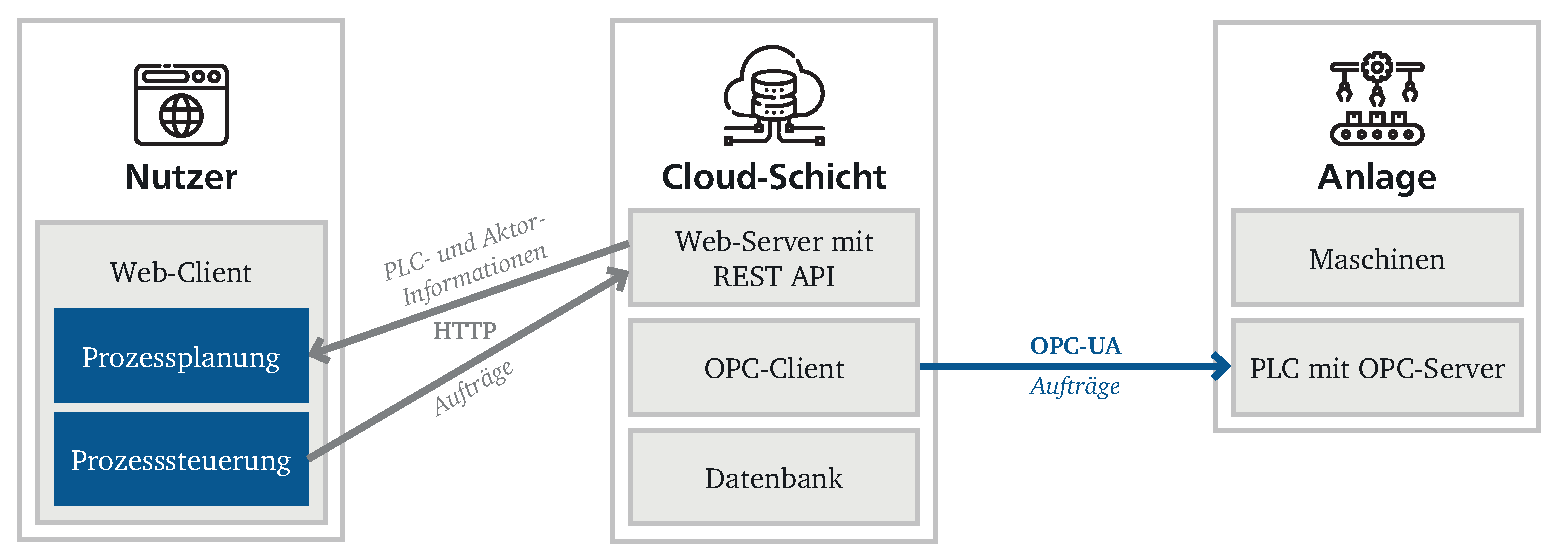
\includegraphics[width=1.0\textwidth]{images/04/dtaInfrastruktur.eps}
    \caption{Kommunikations-Infrastruktur mit Prozessplanungs und -steuerungs Komponenten}
    \label{fig:dtaInfrastruktur}
\end{figure}

Zuletzt bleibt nur noch, eine Authentifizierung und Verschlüsselung hinzuzufügen. Letzteres ist mit wenig Aufwand getan, indem für die Übertragung zwischen dem Browser des Benutzers und der REST API über HTTPS stattfindet und damit wie in Kapitel \ref{subsec:http_https} über TLS verschlüsselt ist; eine unverschlüsselte Übertragung über HTTP wird über die Web-Server Konfiguration verboten. Die Nachrichten, welche über OPC-UA von der Cloud-Schicht zur PLC gesendet werden, sind außerdem über die OPC-UA interne Verschlüsselung gesichert.\\
Die Authentifizierung dagegen wird über die API in der Cloud-Schicht gehandhabt. So muss jeder Nutzer erst einen gültigen API-Key von der REST API erhalten, und diesen dann bei jeder folgenden Nachricht mitsenden. Die API gibt einen solchen Key nur nach einer erfolgreichen Authentifizierungs-Anfrage zurück. Jeder Key ist nutzerspezifisch – und damit auf den Nutzer zurückführbar, falls er verloren gehen sollte – und nur für eine begrenzte Zeit gültig. Die Liste von registrierten Nutzern mit ihren aktuellen gültigen Keys werden dabei innerhalb der Datenbank in der Cloud-Schicht gespeichert.
